%% -*- coding: utf-8 -*-   
\documentclass[12pt,a4paper,headsepline,bibtotoc,twoside]{scrbook}

\usepackage[T1]{fontenc}
\usepackage{ucs}
\usepackage[utf8x]{inputenc} 
\usepackage{lmodern}
%\usepackage{textcomp}
\usepackage{garamond}
\usepackage{helvet}
\usepackage{color}
 
\definecolor{dkgreen}{rgb}{0,0.6,0}
\definecolor{gray}{rgb}{0.5,0.5,0.5}
\definecolor{mauve}{rgb}{0.58,0,0.82}

\definecolor{rltbrightred}{rgb}{1,0,0}
\definecolor{rltred}{rgb}{0.75,0,0}
\definecolor{rltdarkred}{rgb}{0.5,0,0}
%
\definecolor{rltbrightgreen}{rgb}{0,0.75,0}
\definecolor{rltgreen}{rgb}{0,0.5,0}
\definecolor{rltdarkgreen}{rgb}{0,0,0.25}
%
\definecolor{rltbrightblue}{rgb}{0,0,1}
\definecolor{rltblue}{rgb}{0,0,0.75}
\definecolor{rltdarkblue}{rgb}{0,0,0.5}

\definecolor{webred}{rgb}{0.5,.25,0}
\definecolor{webblue}{rgb}{0,0,0.75}
\definecolor{webgreen}{rgb}{0,0.5,0}
\definecolor{webbrightgreen}{rgb}{0,0.5,0}

\usepackage{listings}
\lstset{ %
  language=Python,                % the language of the code
  basicstyle=\footnotesize,           % the size of the fonts that are used for the code
  numbers=left,                   % where to put the line-numbers
  numberstyle=\footnotesize,          % the size of the fonts that are used for the line-numbers
  stepnumber=2,                   % the step between two line-numbers. If it's 1, each line 
                                  % will be numbered
  numbersep=5pt,                  % how far the line-numbers are from the code
  backgroundcolor=\color{white},      % choose the background color. You must add \usepackage{color}
  showspaces=false,               % show spaces adding particular underscores
  showstringspaces=false,         % underline spaces within strings
  showtabs=false,                 % show tabs within strings adding particular underscores
  frame=single,                   % adds a frame around the code
  tabsize=2,                      % sets default tabsize to 2 spaces
  captionpos=b,                   % sets the caption-position to
                                % bottom 
  breaklines=true,                % sets automatic line breaking
  breakatwhitespace=false,        % sets if automatic breaks should only happen at whitespace
  title=\lstname,                   % show the filename of files included with \lstinputlisting;
                                  % also try caption instead of title
  numberstyle=\tiny\color{gray},        % line number style
  keywordstyle=\color{blue},          % keyword style
  commentstyle=\color{dkgreen},       % comment style
  stringstyle=\color{mauve},         % string literal style
  escapeinside={\%*}{*)},            % if you want to add a comment within your code
  morekeywords={*,...}               % if you want to add more keywords to the set
} 
\usepackage[dvips]{thumbpdf}
\usepackage[pdftex,
colorlinks=true,
urlcolor=rltblue,               % \href{...}{...}
anchorcolor=rltbrightblue,
filecolor=rltgreen,             % \href*{...}
linkcolor=rltblue,               % \ref{...} and \pageref{...}
menucolor=webdarkblue,
citecolor=webbrightgreen,
pdftitle={Trabalho Individual},
pdfauthor={Pedro Miguel Clemente Dias Moreira},
pdfsubject={Interac\c{c}\~{a}o Pessoa-Computador},
pdfkeywords={usabilidade, eug\'{e}nio},
% pdfadjustspacing=1,
pagebackref=false,
pdfpagemode=None,
bookmarksopen=true]{hyperref}
\pdfcompresslevel=9

\usepackage[pdftex]{graphicx}
\usepackage{thumbpdf}

%%%%%%%%%%%%%%%%%%%%%%%%%

%% escrita em portugues
%\usepackage[latin1]{inputenc}
\usepackage[portuges]{babel}

% virgulas numericas correctas
\usepackage{icomma}

% processamento com indicação de linhas pelo pacote xdvi
\usepackage{srcltx}

\bibliographystyle{plain}

%% introducao do ambiente de geracao de indices
\usepackage{makeidx}

\usepackage[isu,small,ruled]{caption}
\setlength{\captionmargin}{0.5cm}
\usepackage{prettyref}

%\usepackage[portuges]{minitoc}

%% pacotes matematicos AMS
\usepackage[intlimits]{amsmath}
\usepackage{amssymb}

% simbolos matematicos
%\usepackage{jeffe}
%% graficos com dvips
%%
%%
%%
%% as fontes para os graficos são de 12pt, helvetica
% \usepackage[dvips]{graphics}
\usepackage{lscape}
\usepackage{subfigure}

% captions
\usepackage{float}
\usepackage{rotating}

\setlength{\topmargin}{0cm}
\setlength{\headsep}{0cm}

%% bibliografia por temas e capitulos
%\usepackage{bibtopic}

%% especificacoes para portugues
\newrefformat{teorema}{Teorema~\ref{#1}}
\newrefformat{cha}{Cap{\'\i}tulo~\ref{#1}}
\newrefformat{sec}{Sec{\c c}{\~a}o~\ref{#1}}
\newrefformat{tab}{Tab.~\ref{#1}}
\newrefformat{eq}{Eq.~\ref{#1}}
\newrefformat{def}{Def.~\ref{#1}}
%% na p{\'a}g. #2}
\newrefformat{fig}{Fig.~\ref{#1}}
%% na p{\'a}g. #2}
\newrefformat{alg}{Alg.~\ref{#1}}
\newrefformat{pag}{P{\'a}g.~\ref{#1}}

\newtheorem{assuncao}{Assun{\c c}{\~a}o}
\newtheorem{definicao}{Defini{\c c}{\~a}o}
\newtheorem{teorema}{Teorema}

\newcommand{\goodgap}{%
\hspace{\subfigtopskip}%
\hspace{\subfigbottomskip}}

\newcommand\glossaryname{Gloss{\'a}rio}

% processamento mais agradável de figuras
\renewcommand{\topfraction}{0.85}
\renewcommand{\textfraction}{0.1}
\renewcommand{\floatpagefraction}{0.75}

%%% fontes para cabecalhos e inicios de capitulos
%\renewcommand{\sectfont}{\rmfamily\bfseries}

%\renewcommand{\headfont}{\scshape}


%%% novas declaracoes para amsmath.sty
%\DeclareMathOperator{\argmax}{argmax}
\def\argmax{\operatornamewithlimits{arg\,max}}
\DeclareMathOperator{\tgh}{tgh}
\DeclareMathOperator{\arctg}{arctg}
\DeclareMathOperator{\arcsen}{arcsen}
\DeclareMathOperator{\sen}{sen}
\DeclareMathOperator{\erf}{erf}
\DeclareMathOperator{\ud}{d}
\DeclareMathOperator{\jacobian}{J}
\DeclareMathOperator{\abs}{abs}
\DeclareMathOperator{\cov}{cov}
\DeclareMathOperator{\signum}{sgn}
\DeclareMathOperator{\decibel}{dB}
\DeclareMathOperator{\pixel}{pixel}
\DeclareMathOperator{\verdade}{\mathbf{Verdade}}
\DeclareMathOperator{\falso}{\mathbf{Falso}}
\DeclareMathOperator{\probcdf}{Pr}


%%
\usepackage{supertabular}

% posicionamento arbitrario de texto
\usepackage[absolute]{textpos}
\usepackage{type1cm}
\usepackage{lettrine}
\usepackage{multind}
%\makeindex{aut}
%\makeindex{alf}

\begin{document}

\garamond
%% modos de armazenamento de imagens em Postscript encapsulado
%% e comprimido
\DeclareGraphicsRule{eps.gz}{eps}{eps.bb}{`gunzip -c #1}
%% directoria onde se armazena os ficheiros
\graphicspath{{EPS/}}

%% \symbol{64} corresponde a @
%% parte frontal da tese
\frontmatter
%\maketitle
\thispagestyle{empty}
\begin{titlepage}
  \vspace*{2cm}
  \baselineskip=24pt
  % printing UNIVERSITY LOGO
  \textblockorigin{-18pt}{-2pt}
  \begin{textblock*}{10cm}(2cm,1cm)
    
\includegraphics[width=3.5cm]{LOGO_IPB.png}
  \end{textblock*}
    % printing THESIS LOGO
  \textblockorigin{-18pt}{-2pt}
  \begin{textblock*}{18cm}(3.5cm,2.5cm)
    \centering
    \textbf{{\large INSTITUTO POLITÉCNICO DE BEJA}}
  \end{textblock*}

  % \textblockorigin{-18pt}{-2pt}
  % \begin{textblock*}{18cm}(3.5cm,3.5cm)
  %   \centering
  %   \textbf{{\large ESCOLA SUPERIOR DE TECNOLOGIA E GESTÃO}}
  % \end{textblock*}

  \textblockorigin{0cm}{3.5cm}
  \begin{textblock*}{13cm}(3.6cm,2cm)
    \centering
    %\includegraphics[height=4cm]{figuras/respmix2d}
  \end{textblock*}

   \textblockorigin{0cm}{5cm}
   \begin{textblock*}{16cm}(2.5cm,5.5cm)
     \centering
       \textbf{{\large Interacção Pessoa-Computador}}
   \end{textblock*}


   \textblockorigin{0cm}{5cm}
   \begin{textblock*}{16cm}(2.5cm,8.4cm)
     \centering
       \textbf{{\large Pedro Miguel Clemente Dias Moreira, 10015\\}}
   \end{textblock*}

   \textblockorigin{0cm}{5cm}
   \begin{textblock*}{16cm}(2.5cm,12cm)
     \centering
       \textbf{{\large Trabalho Individual 1}}
   \end{textblock*}

   \textblockorigin{0cm}{5cm}
   \begin{textblock*}{16cm}(2.5cm,15.2cm)
     \centering
       \textbf{\large Engenharia Informática}
   \end{textblock*}

   \textblockorigin{0cm}{5cm}
   \begin{textblock*}{16cm}(2.5cm,18.4cm)
     \centering
       \textbf{\large}
   \end{textblock*}

   \textblockorigin{0cm}{5cm}
   \begin{textblock*}{16cm}(2.5cm,21.2cm)
     \centering
       \textbf{20 de Março 2012}
   \end{textblock*}
   
\end{titlepage}
%%
%% capa.tex
%% 
%% Made by Jose Jasnau Caeiro
%% Login   <jasnau@isolda>
%% 
%% Started on  Fri Jul 31 11:30:46 2009 Jose Jasnau Caeiro
%% Last update Fri Jul 31 11:30:46 2009 Jose Jasnau Caeiro
%%

\thispagestyle{empty}
\cleardoublepage


%% corpo do livro
\mainmatter
%% realizacao de miniindices de conteudo


\cleardoublepage
\pagestyle{headings}
\setcounter{page}{1}
\pagenumbering{roman}
%\addcontentsline{toc}{section}{Contents}
\addcontentsline{toc}{section}{Índice Geral}
\tableofcontents
\cleardoublepage
 \addcontentsline{toc}{section}{Lista de Figuras}
 \listoffigures
 \cleardoublepage
 \addcontentsline{toc}{section}{Lista de Tabelas}
 \listoftables
 \cleardoublepage
%% \include{listasimbolos}
\cleardoublepage


%\pagestyle{headings}
\setcounter{page}{1}
\pagenumbering{arabic}

%%\part{}
\thispagestyle{plain}
\chapter{Introdução}
%\label{chap:intro}

\subsubsection*{Objeto do Estudo}
\label{sec:estudo}
O documento apresenta um estudo sobre a usabilidade da aplicação Eugénio. 
São apresentadas \textsc{duas falhas de usabilidade} que vão contra as \textit{regras de blabla}

\subsubsection{Trabalho do Autor}

\subsubsection*{Estrutura do Documento}

\cleardoublepage
\chapter{Teoria}

A sequência dos números de Fibonacci pode ser representada por:
\begin{eqnarray}
  \label{eq:eq1}
  F(n) = \left\{ 
    \begin{array}{ll}
      0 & \,\,\, \text{se}\,\,\, n = 0;\\
      1 & \,\,\, \text{se}\,\,\, n = 1; \\
      F(n-2) + F(n-1) & \,\,\,\text{outros}
    \end{array}
    \right.
\end{eqnarray}


\section{Introdução}
\section{Complexidade Computacional}
\section{Conclusões}

\cleardoublepage


\lstinputlisting[language=Python]{testerec.py}

As minhas conclusões.
\lstinputlisting[language=Python]{fibo.py}

\begin{equation}
  \label{eq:esq1}
  \sqrt{\frac{1}{2}} \times f(x) = 12 \beta \sqrt{3}.
\end{equation}

\begin{figure}
  \centering
  
\includegraphics[width=5cm]{2000px-Coat_of_arms_of_Portugal_(Lesser).png}
  \caption{Uma bela figura.}
  \label{fig:bela}
\end{figure}


\chapter{Resultados Experimentais}

\section{Introdução}
\section{Protocolo Experimental}
\lstinputlisting[language=C]{teste.c}
\section{Análise dos Resultados Experimentais}

\begin{figure}
  \centering
  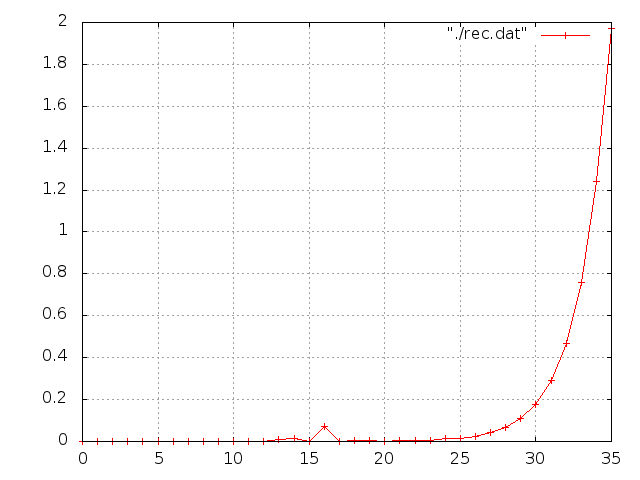
\includegraphics[width=14cm]{teste.png}
  \caption{Os resultados experimentais para o algoritmo iterativo.}
  \label{fig:rec}
\end{figure}
\section{Conclusões}
Os resultados experimentais apontam para que a complexidade algorítimica seja do tipo $O(n)$. Na \prettyref{tab:execucao} apresentam-se os resultados experimentais para alguns valores de $n$. 

Encontram-se em (Tiobe Index, 2012)\cite{09:_tiobe_progr_commun_index} as estatísticas sobre a utilização das diversas linguagens de programação.
\begin{table}
  \centering
  \begin{tabular}{c|c}
    N & tempo de execução (seg) \\ \hline
0 & 0.0 \\
1 & 0.0 \\
2 & 0.0 \\
3 & 0.0 \\
4 & 0.0 \\
5 & 0.0 \\
6 & 0.0 \\
7 & 0.0 \\
8 & 0.0 \\
9 & 0.0 \\
10 & 0.0 \\
11 & 0.0 \\
12 & 0.0 \\
13 & 0.008 \\
14 & 0.012001 \\
15 & 0.0 \\
16 & 0.072004 \\
17 & 0.0 \\
18 & 0.004 \\
19 & 0.004001 \\
20 & 0.0 \\
21 & 0.004 \\
22 & 0.004 \\
23 & 0.004 \\
24 & 0.012001 \\
25 & 0.016001 \\
26 & 0.024002 \\
27 & 0.044002 \\
28 & 0.068005 \\
29 & 0.112007 \\
30 & 0.176011 \\
31 & 0.292018 \\
32 & 0.468029 \\
33 & 0.760047 \\
34 & 1.240078 \\
35 & 1.972123
  \end{tabular}
  \caption{Uma tabela de tempos de execução.}
  \label{tab:execucao}
\end{table}

\chapter{Conclusões}
\label{chap:conclu}

\subsubsection{Complexidade}
Este documento sucks. A programação em Python apresenta o potencial
de ser utilizada em contextos perigosos (Seitz, 2009) \cite{seitz09:_gray_hat_python}.

\subsubsection{Perspetivas Futuras}
Desenvolvimento de software eficiente. Exemplos de programação com
funções recursivas a evitar.

\bibliography{estudo}

\end{document}
